\section{Offline passive testing}
\label{sec:testing:offpassive}

In this section, we tackle the problem of testing industrial
systems (as described in the previous chapter), without
disturbing them, and without having any specification. Those two
constraints sounds familiar as they have already been taken into
consideration in the previous chapter.

Manual testing is, by far, the most popular technique for
testing, but this technique is known to be error-prone as well.
Additionally, production systems are usually composed of
thousands of states (i.e. sets of conditions that exist at a
given instant in time) and production events, which makes
testing time consuming. Our industrial partner Michelin is a
worldwide tire manufacturer that designs most of its factories,
production systems, and software by itself. In a factory, there
are different workshops for each step of the tire building
process. At a workshop level, we observe a continuous stream of
products from specific entry points (railroad switches) to a
finite set of exit points, constituting production lines.
Thousands of \emph{production events} are exchanged among the
industrial devices of the same workshop every day, allowing some
factories to build over 30,000 tires a day.

In this context, we propose a testing framework for production
systems that is composed of two parts: a model inference engine
as described in Chapter \ref{sec:modelinf:prodsystems}, and a
passive testing engine, which will be presented in this section.
Both parts have to be fast and scalable to be used in practice.
The main idea of our proposal is that, given a running production
system, we extract knowledge and models by passively monitoring
it. Such models describe the functional behaviours of the system,
and may serve for different purposes, e.g., testing of a second
production system. The latter can be a new system roughly
comparable to the first one in terms of features, but it can also
be an updated version of the first one. Indeed, upgrades might
inadvertently introduce or create faults, and could lead to
severe damages. Here, testing the updated system means detecting
potential regressions before deploying changes in production.

A \textit{passive tester} (a.k.a. observer) aims at checking
whether a system under test conforms to an inferred model in
offline mode. \textit{Offline testing} means that a set of
traces has been collected while the system is running. Then, the
tester gives verdicts.
We collect the traces of the system under test by reusing some
parts of the model inference engine, and we build a set of traces
with the same level of abstraction as those considered for
inferring models. Then, we use these traces to check if the
system under test conforms to the inferred models.  Conformance
is defined with two implementation relations, which express
precisely what the system under test should do. The first
relation corresponds to the trace preoder \cite{DNH84}, which is
a well-known relation based upon trace inclusion, and heavily
used with passive testing.  Nevertheless, our inferred models are
partials, i.e.  they do not necessarily capture all the possible
behaviours that should happen. That is why we propose a second
implementation relation, less restrictive on the traces that
should be observed from the system under test.

In the next section, we describe a better solution to segment and
filter the initial trace set given as input. Indeed, with the
statistical analysis introduced in
\crossref{sec:modelinf:prodsystems}{sec:modelinf:prodsystems:segmentation},
we hit several problems, mainly because our algorithm was not
stable, i.e. the use of a configurable minimum limit was not
accurate enough. In Section \ref{sec:testing:offpassive:normal},
we introduce a new step of the model inference method described
in Chapter \ref{sec:modelinf:prodsystems} that is required to
enable testing. Then, we present our offline passive testing
technique on-top of this model inference method in Section
\ref{sec:testing:offpassive:testing}. We present key results in
Section \ref{sec:testing:offpassive:impl-exp}, and we conclude on
this work in Section \ref{sec:testing:offpassive:conclusion}.

\textbf{Publication.} This work has been published in the
Proceedings of the 13th International Conference on Formal
Methods and Models for Co-Design (MEMOCODE'15).

%%%%%%%%%%%%%%%%%%%%%%%%%%%%%%%%%%%%%%%%%%%%%%%%%%%%%%%%%%%%%%%%%

\subsection{A better solution to trace segmentation and filtering}

In
\crossref{sec:modelinf:prodsystems}{sec:modelinf:prodsystems:segmentation},
we presented a statistical analysis to segment and filter the
initial trace set used to infer models. However, this method was
not stable, and we decided to rework it. We now rely on a machine
learning technique to segment it into several subsets, one per
entry point of the system $\mathit{Sua}$. We leverage this
process to also remove incomplete traces, i.e. traces that do not
express an execution starting from an entry point and ending to
an exit point. These can be extracted by analysing the traces and
the variable $point$, which captures the product physical
location.

In order to determine both entry and exit points of
$\mathit{Sua}$, we rely on an outlier detection approach
\cite{1695852}. An outlier is an observation which deviates so
much from the other observations as to arouse suspicions that it
was generated by a different mechanism. More precisely, we chose
to use the \textit{k-means clustering} method, a machine learning
algorithm, which is both fast and efficient, and does not need to
be trained before being effectively used (that is called
unsupervised learning, and it is well-known in the machine
learning field). \textit{k-means clustering} aims to partition
$n$ observations into $k$ clusters.  Here, observations are
represented by the variable $point$ present in each trace of
$Traces({Sua})$, which captures the product physical location,
and $k=2$ as we want to group the outliers together, and leave
the other points in another cluster. But, since we want to
leverage the largest part of the initial trace set, we apply
\textit{k-means clustering} several times until reaching 80\% of
traces retained.

Once the entry and exit points are found, we segment
$Traces({Sua})$ and obtain a set $CTraces({Sua})=\{ST_1, \dots,
ST_n\}$. Then, we apply the same generation and reduction steps
as described in
\crossref{sec:modelinf:prodsystems}{sec:modelinf:prodsystems:generation}
and
\crossref{sec:modelinf:prodsystems}{sec:modelinf:prodsystems:reduction}
so that we obtain the reduced model $R(\EuScript{S}) =
\{R(\EuScript{S}_1),\dots,R(\EuScript{S}_n)\}$.

\subsection{Extending inferred models with normalisation}
\label{sec:testing:offpassive:normal}

In order to perform testing, we reuse the reduced model
$R(\EuScript{S}) = \{R(\EuScript{S}_1),\dots,R(\EuScript{S}_n)\}$
inferred with Autofunk that we \textit{normalise} to get rid of
some runtime-dependent information.  Indeed, both models
$\EuScript{S}$ and $R(\EuScript{S})$ include parameters that are
dependent to the products being manufactured.  That is a
consequence of generating models that describe behaviours of a
continuous stream of products which are strictly identified, i.e.
for each action in a given sequence, we have the assignment $(pid
= val)$ ($pid$ stands for product identifier).  Here, we
normalise these models before using them for testing.  The
resulting models are denoted with $\EuScript{S}^{N}$ and
$R(\EuScript{S}^{N})$.

We remove the assignments relative to product identifiers and
timestamps. Furthermore, we label all the final locations with
"Pass". We denote these locations as verdict locations and gather
them in the set $Pass \subseteq L_{\EuScript{S_i}^{N}}$. Both
$\EuScript{S}^{N}$ and $R(\EuScript{S}^{N})$ represent more
generic models, i.e.  they express \textit{some possible
behaviours that should happen}. These behaviours are represented
by the traces $Traces_{Pass} (\EuScript{S}^{N})=\displaystyle
\bigcup_{1 \leq i \leq n} Traces_{Pass}
(\EuScript{S}_i^{N})=Traces_{Pass} (R(\EuScript{S}^{N}))$. We
refer to these traces as \textit{pass traces}. We call the other
traces \textit{possibly fail traces}.

%%%%%%%%%%%%%%%%%%%%%%%%%%%%%%%%%%%%%%%%%%%%%%%%%%%%%%%%%%%%%%%%%

\subsection{Offline passive testing with Autofunk}
\label{sec:testing:offpassive:testing}

\begin{figure}[ht]
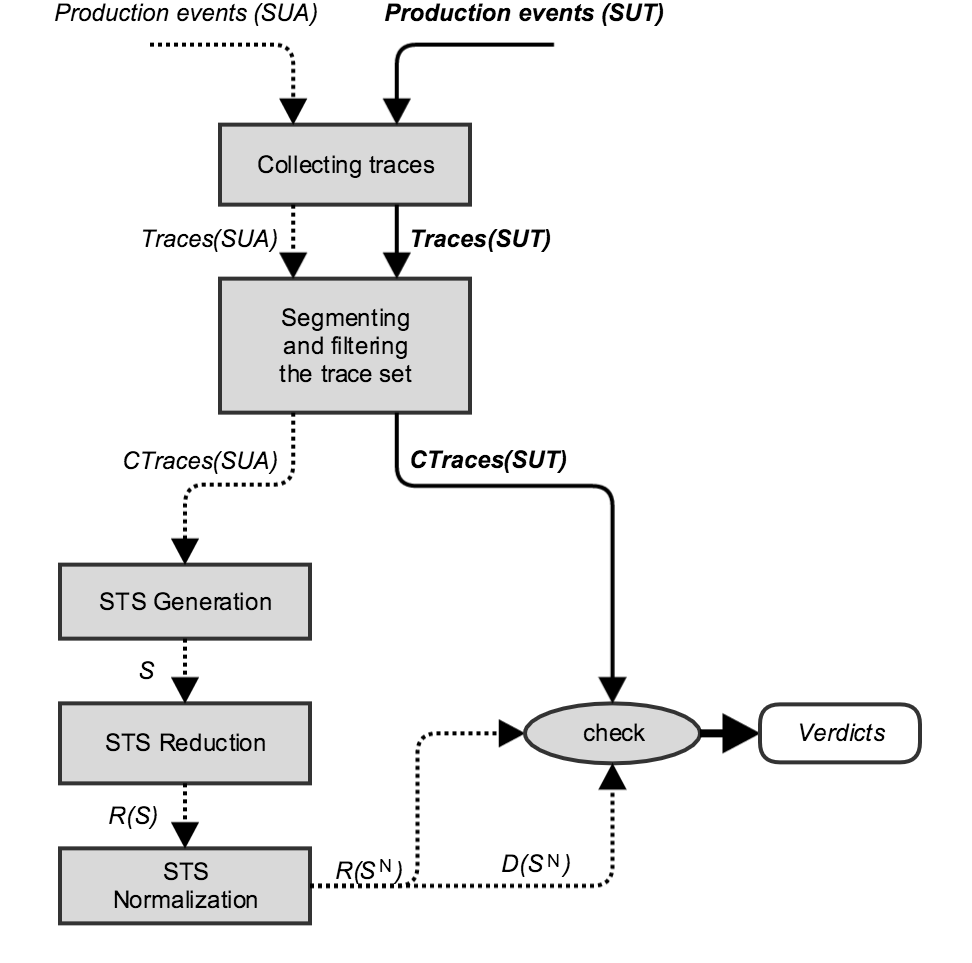
\includegraphics[width=0.85\linewidth]{figures/passive_autofunk.png}

\caption{Autofunk's testing architecture}
\label{fig:passive-autofunk}
\end{figure}

We consider both models $\EuScript{S}^{N}$ and
$R(\EuScript{S}^{N})$ of a system under analysis $\mathit{Sua}$,
generated by our inference-based model generation framework, as
reference models. In this section, we present the second part of
our framework, dedicated to the passive testing of a system under
test $\mathit{Sut}$. As depicted in Figure
\ref{fig:passive-autofunk}, the passive testing of $\mathit{Sut}$
is performed offline, i.e. a set of production events has been
collected beforehand from $\mathit{Sut}$, in the same way as for
$\mathit{Sua}$. These are grouped into traces to form the trace
set $Traces({Sut})$. The latter is filtered as described in
Section \ref{part2:segmentation} to obtain a set of complete
traces denoted with $CTraces({Sut})$.  We then perform passive
testing to check if $\mathit{Sut}$ conforms to
$\EuScript{S}^{N}$. Below, we define conformance with
implementation relations, and provide a passive testing algorithm
that aims to check whether these relations hold.

\subsubsection{Implementation relations and verdicts}

%The specification considered for passive testing is here the previous inferred models $\EuScript{S}^{N}$ and $R(\EuScript{S}^{N})$.

Our industrial partner wishes to check whether every complete
execution trace of $\mathit{Sut}$ matches a behaviour captured by
$\EuScript{S}^{N}$. In this case, the test verdict must reflect a
successful result. On the contrary, if an execution of $\mathit{Sut}$ is
not captured by $\EuScript{S}^{N}$, one cannot conclude that
$\mathit{Sut}$ is faulty because $\EuScript{S}^{N}$ is a partial model,
and it does not necessarily includes all the correct
behaviours. Below, we formalise theses verdict notions with two
implementation relations. Such relations between models can only be written
by assuming the following classical test assumption: the
black-box system $\mathit{Sut}$ can be described by a model, here
with a LTS as defined in
\crossref{sec:definitions}{sec:definitions:sts}. We also denote
this model with $\mathit{Sut}$.

The first implementation relation, denoted with $\leq_{ct}$,
refers to the trace preorder relation \cite{DNH84}. It aims at
checking whether all the complete execution traces of
$\mathit{Sut}$ are pass traces of
$\EuScript{S}^{N}=\{\EuScript{S}_1^{N},\dots,\EuScript{S}_n^{N}\}$.
The first implementation relation can be written with the
following definition:

\begin{definition}
\label{rel:impl1}
Let $\EuScript{S}^{N}$ be an inferred model of $\mathit{Sua}$ and
$\mathit{Sut}$ be the system under test. When $\mathit{Sut}$ produces complete
traces also captured by $\EuScript{S}^{N}$, we write:
${Sut} \leq_{ct} \EuScript{S}^{N} =_{def} CTraces({Sut}) \subseteq  Traces_{Pass}(\EuScript{S}^{N})$.
\end{definition}

Pragmatically, the reduced model $R(\EuScript{S}^{N})$ sounds
more convenient for passively testing $\mathit{Sut}$ since it is
strongly reduced in terms of size compared to $\EuScript{S}^{N}$.
The test relation can also be written as below since both models
$\EuScript{S}^{N}$ and $R(\EuScript{S}^{N})$ are trace equivalent:

\begin{proposition}
\label{rel:impl12}
${Sut} \leq_{ct} \EuScript{S}^{N} \text{ iff } CTraces({Sut}) \subseteq  Traces_{Pass}(R(\EuScript{S}^{N}))$
\end{proposition}

As stated previously, the inferred model $\EuScript{S}^{N}$ of
$\mathit{Sua}$ is partial, and might not capture all the
behaviours that should happen on $\mathit{Sut}$. Consequently,
our partner wants a weaker implementation relation, which is less
restrictive on the traces that should be observed from
$\mathit{Sut}$.  Intuitively, this second relation aims to check
that, for every complete trace $t=a_1(\alpha_1)...a_m(\alpha_m)$
of $\mathit{Sut}$, we also have a set of traces of
$Traces_{Pass}(\EuScript{S}^{N})$ having the same sequence of
symbols such that every variable assignment $\alpha_j(x)_{(1 \leq
j \leq m)}$ of $t$ is found in one of the traces of
$Traces_{Pass}(\EuScript{S}^{N})$ with the same symbol $a_j$.
If we take back the example of Figure \ref{fig:firstmodel}, the
trace $t=(17011(nsys=1,nsec=8,point=1,pid=1)\text{ }
17021(nsys=1,nsec=8,point=4,tpoint=9,pid=1)$ is not a pass trace
of $\EuScript{S}^{N}$ because this trace cannot be extracted from
one of the paths of the STS of Figure \ref{fig:firstmodel}, on
account of the variables $point$ and $tpoint$, which do not take
the expected values. However, both variables are assigned with
$point=4,tpoint=9$ in the second path. This is interesting as it
indicates that such values may be correct since they are actually
used in a similar action in a similar path. Here, the second
implementation relation aims at expressing that this trace $t$
captures a correct behaviour as well.

% \begin{comment}
% This second implemenation relation, denoted with $\leq_{mct}$, is written
% with the classes of equivalent paths $[b]$, found in a STS of
% $\EuScript{S}^{N}=\{\EuScript{S}_1^{N},...,\EuScript{S}_n^{N}\}$.
% Indeed, an equivalent class $[b]$ of $\EuScript{S}_i^{N}$ gathers
% STS paths having the same sequence of labels but with
% different guards. The definition of $\leq_{mct}$, given below,
% means that for a trace $t$, an equivalence class $[b]$ must be
% found such that for every valued action $a_j(\alpha_j)$, each
% variable assignment $\alpha_j(x)$ with $x$ a variable, must
% satisfies at least on the guards $G_{j1},...,G_{jk}$ found on
% the transitions labelled with $a_j(p_j)$:
%
% \begin{proposition}
%     Let $\mathit{Sua}$ be the system under analysis,
%     $\EuScript{S}^{N}=\{\EuScript{S}_1^{N},\dots,\EuScript{S}_n^{N}\}$ be its inferred model and $\mathit{Sut}$ be the system under test.
%     We denote ${Sut} \leq_{mct} \EuScript{S}^{N} =_{def} \forall t=
%     a_1(\alpha_1)...a_m(\alpha_m) \in CTraces({Sut}), \exists
%     \EuScript{S}_i^{N} \text{ and } [b]=\{l0_{\EuScript{S}_i^{N}} \xRightarrow{(a_1(p_1),G_{1o}),...,(a_m(p_m),G_{mo})}l_{mo} (1 \leq o \leq k) \}$ such that $\forall \alpha_j(x) (1 \leq j \leq m), \alpha_j(x) \models G_{j1} \vee ... \vee  G_{jk}$ and $l_{mo} \in Pass$.
% \end{proposition}
%
% This relation can be reformulated with the reduced model
% $R(\EuScript{S}^{N})=\{R(\EuScript{S}_1^{N}),\dots,R(\EuScript{S}_n^{N})\}$,
% which reduces the equivalence classes $[b]$ into one STS path.
% Given a trace $a_1(\alpha_1)...a_m(\alpha_m)$, the relation can
% be now written with matrices of guards: for every valued action
% $a_j(\alpha_j)$, each variable assignment $\alpha_j(x)$ must now
% satisfies one of the guards of the matrix line $j$ in
% $M_{[b]}[j,*]$.  If, we take back the trace example
% $t=(17011(nsys=1,nsec=8,point=1,pid=1)\text{ }
% 17021(nsys=1,nsec=8,point=4,tpoint=9,pid=1)$, and the STS of
% Figure \ref{fig:reduced-model}, the assignment $point=4$, which
% is given with the second valued action of $t$, satisfies one of
% the guards of the second line of the matrix $M_{[b]}$.
% \end{comment}

This implementation relation, denoted with $\leq_{mct}$, is
written with:

\begin{definition}
	\label{impl21}
	 Let $\EuScript{S}^{N}$ be an inferred model of $\mathit{Sua}$ and
	 $\mathit{Sut}$ be the system under test.
	We denote ${Sut} \leq_{mct} \EuScript{S}^{N} =_{def} \forall t=
	a_1(\alpha_1) \dots a_m(\alpha_m) \in CTraces({Sut}), \forall \alpha_j(x)_{(1 \leq j \leq m)},\\ \exists \EuScript{S}_i^{N} \in \EuScript{S}^{N} \text{ and } t'\in Traces_{Pass}(\EuScript{S}_i^{N})$ such that $t'=a_1(\alpha_1')...a_m(\alpha_m')$ \text{ and } $\alpha_j'(x)=\alpha_j(x)$.
\end{definition}

In the following, we rewrite this relation in an equivalent but
simpler form. According to the above definition, the successive
symbols and variable assignments of a trace $t \in
CTraces({Sut})$ must be found into several traces of
$Traces_{Pass}(\EuScript{S}_i^{N})$, which have the same sequence
of symbols $a_1...a_m$ as the trace $t$. The reduced model
$R(\EuScript{S}_i^{N})$ was previously constructed to capture
all these traces in $Traces_{Pass}(\EuScript{S}_i^{N})$, having
the same sequence of symbols. Indeed, given a STS
$\EuScript{S}_i^{N}$, all the STS paths of $\EuScript{S}_i^{N}$,
which have the same sequence of symbols labelled on the
transitions, are compacted into one STS path $b$ in
$R(\EuScript{S}_i^{N})$ whose transition guards are stored into a
matrix $M_{[b]}$.

If, we take back the trace example
$t=(17011(nsys=1,nsec=8,point=1,pid=1)\text{ }
17021(nsys=1,nsec=8,point=4,tpoint=9,pid=1))$, and the STS of
Figure \ref{fig:reduced-model}, $t$ is a pass trace w.r.t.
$\leq_{mct}$ because each assignment $\alpha_j(x)$ satisfies at
least one guard of the matrix line $j$. For instance, the
assignment $point=4$, which is given with the second valued
action of $t$, satisfies one of the guards of the second line of
the matrix $M_{[b]}$.

Given a trace $a_1(\alpha_1) \dots a_m(\alpha_m) \in CTraces({Sut})$
and a STS path $b$ of $R(\EuScript{S}_i^{N})$ having the same
sequence of symbols $a_1 \dots a_m$, the relation can be now
formulated as follows: for every valued action $a_j(\alpha_j)$,
each variable assignment $\alpha_j(x)$ must satisfies at least
one of the guards of the matrix line $j$ in $M_{[b]}[j,*]$.

The implementation relation $\leq_{mct}$ can then be written with:

\begin{proposition}
	${Sut} \leq_{mct} \EuScript{S}^{N} \text{ iff } \forall t=
	a_1(\alpha_1) \dots a_m(\alpha_m) \in CTraces({Sut}), \exists
	R(\EuScript{S}_i^{N}) \in R(\EuScript{S}^{N)} \text{ and }
	b=l0_{R(\EuScript{S}_i^{N})} \xRightarrow{(a_1(p_1),M_{[b]}[1,c_{[b]}]),\dots,(a_j(p_j),M_{[b]}[j,c_{[b]}])} l_m$ with $(1 \leq c_{[b]} \leq k)$ such that $\forall \alpha_j(x) (1 \leq j \leq m), \alpha_j(x) \models M_{[b]}[j,1] \vee \dots \vee  M_{[b]}[j,k]$ and $l_m \in Pass$.
\end{proposition}

% \begin{comment}
% This second implementation relation, denoted with $\leq_{mct}$, can be written with the reduced model
% $R(\EuScript{S}^{N})=\{R(\EuScript{S}_1^{N}),\dots,R(\EuScript{S}_n^{N})\}$. Indeed, given a STS $\EuScript{S}_i^{N}$, all the STS paths of$\EuScript{S}_i^{N}$, which have the same sequence of symbols labelled on the transitions, are compacted into one STS path $b$ in $R(\EuScript{S}_i^{N})$ whose transition guards are stored into a matrix $M_{[b]}$. Given a trace $a_1(\alpha_1)...a_m(\alpha_m) \in CTraces({Sut})$ and a STS path $b$ of $R(\EuScript{S}_i^{N})$ having the same sequence of symbols $a_1...a_m$, the relation can
% be now formulated as follows: for every valued action
% $a_j(\alpha_j)$, each variable assignment $\alpha_j(x)$ must
% satisfies at least one of the guards of the matrix line $j$ in
% $M_{[b]}[j,*]$.
%
%
%
%
% If, we take back the trace example
% $t=(17011(nsys=1,nsec=8,point=1,pid=1)\text{ }
% 17021(nsys=1,nsec=8,point=4,tpoint=9,pid=1)$, and the STS of
% Figure \ref{fig:reduced-model}, the assignment $point=4$, which
% is given with the second valued action of $t$, satisfies one of
% the guards of the second line of the matrix $M_{[b]}$. Hence, $t$ represents a correct behaviour w.r.t. the STS of
% Figure \ref{fig:reduced-model}.
%
% \begin{definition}
%     ${Sut} \leq_{mct} \EuScript{S}^{N} \text{ iff } \forall t=
%     a_1(\alpha_1)...a_1(\alpha_m),\\ \exists
%     R(\EuScript{S}_i^{N}) \text{ and } l0_{R(\EuScript{S}_i^{N})} \xRightarrow{(a_1(p_1),G_{1}),...,(a_m(p_m),G_{m})} l_m$ such that $\forall \alpha_j(x) (1 \leq j \leq m), \alpha_j(x) \models M_{[b]}[j,1] \vee ... \vee  M_{[b]}[j,k]$ and $l_m \in Pass$.
% \end{definition}
% \end{comment}

The disjunction of guards $M_{[b]}[j,1] \vee \dots \vee
M_{[b]}[j,k]$, found in the matrix $M_{[b]}$, could be simplified
by gathering all the equalities $x==val$ together with
disjunctions for every variable $x$ that belongs to the parameter
set $p_j$. Such equalities can be extracted with the
\textit{Proj} operator (see Definition \ref{}). We
obtain one guard of the form $\bigwedge_{x \in p_j}(x==val_1 \vee
... \vee x==val_k)$. The STS $D(\EuScript{S}_i^{N})$, derived
from $R(\EuScript{S}_i^{N})$, is constructed with this
simplification of guards:

\TODO{missing ref}

%all the variable assignments found in the guards
%$M_{[b]}[j,1],..., M_{[b]}[j,k]$ can be collected with the
%projection operator $Proj_{x}(G)$.

%It is then possible to create
%vectors of guards from the matrices in $R(\EuScript{S}_i)^{G}$ in
%order to express that a trace $t$ can still comply with the
%behaviours found in $R(\EuScript{S}_i)^{G}$, even if it does not
%strictly satisfy all guards of a single branch (i.e. the same
%column in the matrices), but rather the disjunction of the guards
%belonging to the matrices of this branch.

\begin{definition}
    Let $R(\EuScript{S}_i^{N})=<L_R,l0_R,V_R,V0_R,I_R,\Lambda_R,\rightarrow_R>$ be a STS of $R(\EuScript{S}^{N})$. We denote $D(\EuScript{S}_i^{N})$ the STS $ <L_D,l0_D,V_D,V0_D,I_D,\Lambda_D,\rightarrow_D>$ derived from $R(\EuScript{S}_i^{N})$ such that:
\begin{itemize}
    \item $L_D=L_{R}, l0_D=l0_{R}, I_D=I_{R}, \Lambda_D=\Lambda_{R}$,
    \item $V_D, V0_D$ and $\rightarrow_D$ are given by the following inference rule:

				$\frac{
					\begin{matrix}
					b=l0_{R}
					\xRightarrow{(a_1(p_1),M_{[b]}[1,c_{[b]}])\dots (a_m(p_m),M_{[b]}[m,c_{[b]}]}_{\rightarrow_{R}}
					l_{m}\\
					(1 \leq c_{[b]} \leq k) \text{ in } V0_{R}
					\end{matrix}
				}
				{
					\begin{matrix}
					l0_D
					\xRightarrow{(a_1(p_1),M_b[1])\dots (a_m(p_m),M_b[m])}_{\rightarrow_D}
					l_m\\
					V0_D=V0_D \wedge M_b, M_b[j, 1]_{(1\leq j \leq m)} =\\
					 \displaystyle \bigwedge_{x \in p_j} ( Proj_x(M_{[b]}[j, 1]) \vee \dots \vee Proj_x(M_{[b]}[j, k]))


					%\bigvee_{1 \leq k \leq k} Proj_x ((M_{[b]}[j, k])

					\end{matrix}
				}$
  \end{itemize}

    $D(\EuScript{S}^{N})$ denotes the model $\{D(\EuScript{S}_1^{N}),\dots,D(\EuScript{S}_n^{N}) \}$.
\end{definition}


The second implementation relation $\leq_{mct}$ can now be
expressed by:

\begin{proposition}
    ${Sut} \leq_{mct} \EuScript{S}^{N} \text{ iff }\forall t=
    a_1(\alpha_1) \dots a_m(\alpha_m) \in CTraces({Sut}), \exists D(\EuScript{S}_i^{N}) \in D(\EuScript{S}^{N}) \text{ and }
    l0_{D(\EuScript{S}_i^{N})}
    \xRightarrow{(a_1(p_1),G_{1}),\dots,(a_m(p_m),G_{m})} l_m \text{
    such that } \forall \alpha_j (1 \leq j \leq m), \alpha_j \models G_{j}$ and $l_m \in Pass$.
\end{proposition}


$\leq_{cmt}$ now means that a trace of $\mathit{Sut}$ must also
be a pass trace of the model
$D(\EuScript{S}^{N})=(D(\EuScript{S}_1^{N}),\dots,D(\EuScript{S}_n^{N}))$.
Furthermore, this notion of trace inclusion can be formulated
with the first implementation relation $\leq_{ct}$ as follows:

\begin{proposition}
	\label{rel:impl2}
${Sut} \leq_{mct} \EuScript{S}^{N} \text{ iff } CTraces({Sut})\subseteq Traces_{Pass}(D(\EuScript{S}^{N}))$

${Sut} \leq_{mct} \EuScript{S}^{N}\Leftrightarrow {Sut} \leq_{ct} D(\EuScript{S}^{N})$

\end{proposition}

The implementation relation $\leq_{mct}$ is now expressed with the first
relation $\leq_{ct}$, which implies that our passive testing algorithm shall be
the same for both relations but shall take different reference models.

\subsubsection{Passive testing algorithm}

The passive testing algorithm, which aims to check whether the
two previous implementation relations hold, is given in Algorithm
\ref{algo:check}. It takes the complete traces of $\mathit{Sut}$ and the
models $R(\EuScript{S}^{N})$ and $D(\EuScript{S}^{N})$, with
regards to Propositions \ref{rel:impl12} and \ref{rel:impl2}. It
returns the verdict "Pass$\leq_{ct}$" ("Pass$\leq_{mct}$") if the
relation $\leq_{ct}$ is satisfied ($\leq_{mct}$ respectively).

It relies upon the function \textit{checktrace(trace t, STS S)} to check
whether the trace $t=a_1(\alpha_1)...a_m(\alpha_m)$ is also a
trace of the STS $S$. If a STS path $b$ is composed of the same sequence of
symbols as the trace $t$, the function tries to find a matrix
column  $M=M_{[b]}[*,i]$ such that every variable assignment $\alpha_j$
satisfies the guard $M[j]$. If such a column of guards exists,
the function returns True, and False otherwise.

Algorithm \ref{algo:check} covers every trace $t$ of
$CTraces({Sut})$ and tries to find a STS $R(\EuScript{S}_i^{N})$
such that $t$ is also a trace of $R(\EuScript{S}_i^{N})$ with
$check(t, R(\EuScript{S}_i^{N}))$.  If no model
$R(\EuScript{S}_i^{N})$ has been found, the trace $t$ is placed
into the set $T_1$. $T_1$ gathers the possibly fail traces
w.r.t. $\leq_{ct}$. Thereafter, the algorithm performs the same
step but on the STS $D(\EuScript{S}^{N})$. One more time, if no
model $D(\EuScript{S}_i^{N})$ has been found, the trace $t$ is placed
into the set $T_2$.  The latter gathers the possibly fail traces,
w.r.t. the relation $\leq_{mct}$.

Finally, if $T_1$ is empty, the verdict "Pass$\leq_{ct}$" is
returned, which means that the first implementation relation holds.
Otherwise, $T_1$ is provided. If $T_2$ is empty, the verdict
"Pass$\leq_{mct}$" is returned, or $T_2$ in the other case.

\begin{algorithm}[h]
\begin{scriptsize}
    \SetKwInOut{Input}{input}
    \SetKwInOut{Output}{output}
    \SetKwFunction{check}{check}

    \Input{$R(\EuScript{S}^{N})=\{R(\EuScript{S}_1^{N}),...,R(\EuScript{S}_n^{N})\},
    D(\EuScript{S}^{N})=\{D(\EuScript{S}_1^{N}),...,D(\EuScript{S}_n^{N})\}, CTraces({Sut})$}
    \Output{Verdits or possibly fail trace sets $T_1, T_2$ }

$T_1 = T_2 = \emptyset$\;
    \ForEach{$t \in CTraces({Sut})$}{

        \ForEach{$i \in 1, \dots , n$}{

            \lIf{\check($t$, $R(\EuScript{S}_i^{N})$)}{
                break
            }
        }
        \If{$i==n$} {
            $T_1=T_1 \cup \{t\}$

            \ForEach{$i \in 1, \dots , n$}{

                \lIf{\check($t$, $D(\EuScript{S}_i^{N})$)}{
                    break
                }}
            \lIf{$i==n$} {
                $T_2=T_2 \cup \{t\}$
            }

        }

     \lIf{$T_1==\emptyset$} {
        return "Pass$\leq_{ct}$"}
     \lElse{return $T_1$}
     \lIf{$T_2==\emptyset$} {
        return "Pass$\leq_{mct}$"}
     \lElse{return $T_2$}


    }%endfor1

    \BlankLine
    \BlankLine

    \SetKwProg{Fn}{Function}{ is}{end}
    \Fn{check(trace t, STS S ) : bool}{
        \If{$\exists b=l0_{\EuScript{S}}
            \xRightarrow{(a_1(p_1),G_{1},A_{1})\dots (a_n(p_n),G_{n},A_{n})}
            l_n | trace = (a_1, \alpha_1),\dots ,(a_n, \alpha_n)$ and $l_n \in Pass$}{
            $M_{[b]}=Mat(b)$ is the Matrix $k \times m$ of $b$\;
            $i=1$\;
            \While{$i \leq m$}{
                $M=M_{[b]}[*,i]$\;
                \ForEach{$j \in 1, \dots , n$}{
                    \lIf{$\alpha_j \not\models M[j]$}{
                        break
                    }
                }

                \lIf{$j==n$}{
                    return $True$
                }
                $i++$\;
            }


        }
        return $False$\;
}
    \caption{Passive testing algorithm}
    \label{algo:check}
\end{scriptsize}
\end{algorithm}

When one of the implementation relations does not hold, this algorithm
offers the advantage to provide the possibly fail traces of
$CTraces({Sut})$. Such traces can be later analysed to check if
$\mathit{Sut}$ is correct or not. That is helpful for Michelin engineers
as it allows them to only focus on what are potentially faulty
behaviours, reducing debugging time, and making engineers more
efficient.

%%%%%%%%%%%%%%%%%%%%%%%%%%%%%%%%%%%%%%%%%%%%%%%%%%%%%%%%%%%%%%%%%

\subsection{Implementation and experimentation}
\label{sec:testing:offpassive:impl-exp}

We conducted several experiments with real sets of production
events, recorded in one of Michelin's factories at different
periods of time. We executed our implementation on a Linux
(Debian) machine with 12 Intel(R) Xeon(R) CPU X5660 @ 2.8GHz and
64GB RAM.

We present, in Figure \ref{fig:results}, the results of several
experiments on the same production system with different trace
sets, recorded at different periods of time. We focus on the
passive testing component here, but one can find an extensive
evaluation on the model inference part in
\cite{DBLP:conf/debs/SalvaD15}. The first column shows the experiment
number, columns 2 and 3 respectively give the sizes of the trace
sets of the system under analysis $\mathit{Sua}$ and of the system under
test $\mathit{Sut}$. The two next columns show the percentage of pass
traces w.r.t the relations $\leq_{ct}$ and $\leq_{mct}$. The last
column indicates the execution time for the testing phase.

\begin{figure*}
\begin{center}
\begin{tabular}{| c | c | c | c | c | c |}
\hline
Exp. & $Card(Traces({Sua}))$ & $Card(CTraces({Sut}))$ & Pass$\leq_{ct}$ & Pass$\leq_{mct}$ & Time\\
\hline
\hline
$1$ & 2,075 & 2,075 & 100\% & 100\% & 1 \\
\hline
$2$ & 53,996 & 2,075 & 3\% & 30\% & 4\\
\hline
$3$ & 53,996 & 25,047 & 98\% & 98\% & 10\\
\hline
\end{tabular}
\end{center}

    \caption{Results of our passive testing method based on a same specification}
    \label{fig:results}
\end{figure*}

In Experiment $1$, we decided to use the same production events
for both inferring models, i.e. specifications, and testing. This
experiment shows that our implementation
behaves correctly when trace sets are similar, i.e. when
behaviours of both $\mathit{Sua}$ and $\mathit{Sut}$ are equivalent.\\
Experiment $2$ has been run with traces of $\mathit{Sut}$ that are older
than those of $\mathit{Sua}$, which is unusual as the de facto usage of
our framework is to build specifications from a production system
$\mathit{Sua}$, and to take a newer or updated system as $\mathit{Sut}$.
Here, only 30\% of the traces of $\mathit{Sut}$ are pass traces w.r.t.
the second implementation relation (same sequence of symbols with
different values). There are two explanations: the system has
been updated between the two periods of record (4 months), and
production campaigns, i.e. grouping of planned orders and process
orders to produce a certain amount of products over a certain
period of time, were different (revealed by \textit{Autofunk},
indicating that values for some key parameters were unknown).\\
Finally, experiment $3$ shows good results as the specification
models are rich enough, i.e.  built from a larger set of traces
(10 days) than the one collected on $\mathit{Sut}$. Such an experiment
is a typical usage of our framework at Michelin.
The traces of $\mathit{Sut}$ have been collected for 5 days, and
it took only 10 minutes to check conformance. While 98\% of the
traces are pass traces, the remaining 2\% are new behaviours that
never occured before. Such information is essential for Michelin
engineers to determine the root causes. Even though 2\% may
represent a large set to analyse, \textit{Autofunk} improves
their work by highlighting the traces to focus on.
Such subset may contain false positives depending on the
richness of the models, but using large sets of traces to build
the models reduces the number of false positives.

%%%%%%%%%%%%%%%%%%%%%%%%%%%%%%%%%%%%%%%%%%%%%%%%%%%%%%%%%%%%%%%%%

\subsection{Conclusion}
\label{sec:testing:offpassive:conclusion}

In this section, we present a fast offline passive testing
framework combining different fields such as model inference,
expert systems, and machine learning. Such a framework is an
extension of previous works based on model inference, whose name
is Autofunk.

Given a large set of production events, our framework infers
exact models whose traces are included in the initial trace set
of a system under analysis.  Such models are then reused as
specifications to perform offline passive testing, using a second
set of traces recorded on a system under test.  Using two
implementation relations, Autofunk is able to determine what has
changed between the two systems. This is particularly useful for
our industrial partner Michelin since potential regressions can
be detected while deploying changes in production. Initial
results are encouraging, and Michelin engineers see a real
potential in this framework.
